%  article.tex (Version 3.3, released 19 January 2008)
%  Article to demonstrate format for SPIE Proceedings
%  Special instructions are included in this file after the
%  symbol %>>>>
%  Numerous commands are commented out, but included to show how
%  to effect various options, e.g., to print page numbers, etc.
%  This LaTeX source file is composed for LaTeX2e.

%  The following commands have been added in the SPIE class 
%  file (spie.cls) and will not be understood in other classes:
%  \supit{}, \authorinfo{}, \skiplinehalf, \keywords{}
%  The bibliography style file is called spiebib.bst, 
%  which replaces the standard style unstr.bst.  

%%\documentclass[]{spie}  %>>> use for US letter paper
\documentclass[a4paper]{spie}  %>>> use this instead for A4 paper
%%\documentclass[nocompress]{spie}  %>>> to avoid compression of citations
%% \addtolength{\voffset}{9mm}   %>>> moves text field down
%% \renewcommand{\baselinestretch}{1.65}   %>>> 1.65 for double spacing, 1.25 for 1.5 spacing 
%  The following command loads a graphics package to include images 
%  in the document. It may be necessary to specify a DVI driver option,
%  e.g., [dvips], but that may be inappropriate for some LaTeX 
%  installations. 
\usepackage[]{graphicx}
\usepackage{amsmath}
\usepackage{multirow}
\usepackage{url}

\title{Predicting Chroma from Luma with Frequency Domain Intra Prediction}

%>>>> The author is responsible for formatting the 
%  author list and their institutions.  Use  \skiplinehalf 
%  to separate author list from addresses and between each address.
%  The correspondence between each author and his/her address
%  can be indicated with a superscript in italics, 
%  which is easily obtained with \supit{}.

\author{Nathan E. Egge
\skiplinehalf
Mozilla, Mountain View, USA
}

%>>>> Further information about the authors, other than their 
%  institution and addresses, should be included as a footnote, 
%  which is facilitated by the \authorinfo{} command.

%\authorinfo{Further author information: (Send correspondence to A.A.A.)\\A.A.A.: E-mail: aaa@tbk2.edu, Telephone: 1 505 123 1234\\  B.B.A.: E-mail: bba@cmp.com, Telephone: +33 (0)1 98 76 54 32}
%%>>>> when using amstex, you need to use @@ instead of @
 

%%%%%%%%%%%%%%%%%%%%%%%%%%%%%%%%%%%%%%%%%%%%%%%%%%%%%%%%%%%%% 
%>>>> uncomment following for page numbers
% \pagestyle{plain}    
%>>>> uncomment following to start page numbering at 301 
%\setcounter{page}{301} 
 
  \begin{document} 
  \maketitle 

%%%%%%%%%%%%%%%%%%%%%%%%%%%%%%%%%%%%%%%%%%%%%%%%%%%%%%%%%%%%% 
\begin{abstract}
This paper describes a technique for performing intra prediction of the chroma
 planes based on the reconstructed luma plane in the frequency domain.
This prediction exploits the fact that while RGB to YUV color conversion has
 the property that it decorrelates the color planes globally across an image,
 there is still some correllation locally at the block level\cite{LeeCho09}.
Previous proposals compute a linear model of the spatial relationship between
 the luma plane (Y) and the two chroma planes (U and V)\cite{JCTVCB021}.
In codecs that use lapped transforms this is not possible since transform
 support extends across the block boundaries\cite{Tran2003}.
We design a frequency domain intra predictor for chroma that exploits the same
 local correlation with lower complexity than the spatial predictor and which
 works with lapped transforms.


%(need to talk about improvements over other forms of intra prediction)
%(what about complexity, fewer multiplies when predicting the model)
\end{abstract}

%>>>> Include a list of keywords after the abstract 

%\keywords{Manuscript format, template, SPIE Proceedings, LaTeX}
\keywords{Intra Prediction, Lapped Transforms, Color Image Coding, Chroma
 Correlation, Regression}

%%%%%%%%%%%%%%%%%%%%%%%%%%%%%%%%%%%%%%%%%%%%%%%%%%%%%%%%%%%%%
\section{INTRODUCTION}
\label{sec:intro}  % \label{} allows reference to this section

Still image and video codecs typically consider the problem of intra-prediction
 in the spatial domain.
A predicted image is generated on a block-by-block basis using the previously
 reconstructed neighboring blocks for reference, and the residual is encoded
 using standard entropy coding techniques.
Modern codecs use the boundary pixels of the neighboring blocks along with a
 directional mode to predict the pixel values across the current block (e.g.,
 AVC, HEVC, VP8, WebP, etc.).
These directional predictors are cheap to compute (often directly copying pixel
 values or applying a simple linear kernel), exploit local coherency (with low
 error near the neighbors) and predict hard to code features (extending sharp
 directional edges across the block).

%In the Daala video codec, we use a reversible lapped transform to 
In codecs that use lapped transforms these techniques are not applicable (e.g.,
 VC-1, JPEG-XR, Daala, etc.).
The challenge here is that the neighboring spatial image data is not available
 until {\em after} the current block has been decoded and the appropriate
 unlapping filter has been applied across the block boundaries.
Figure \ref{fig:decode} shows the decode pipeline of a codec using lapped
 transforms with a single block size.
The support used in spatial intra prediction is exactly the region that has not
 had the unlapping post-filter applied.
Note that the pre-filter has the effect of decorrelating the image along block
 boundaries so that the neighboring pixel values before unlapping are
 particularly unsuitable for use in prediction.


\begin{figure}
\begin{center}
\begin{tabular}{c}
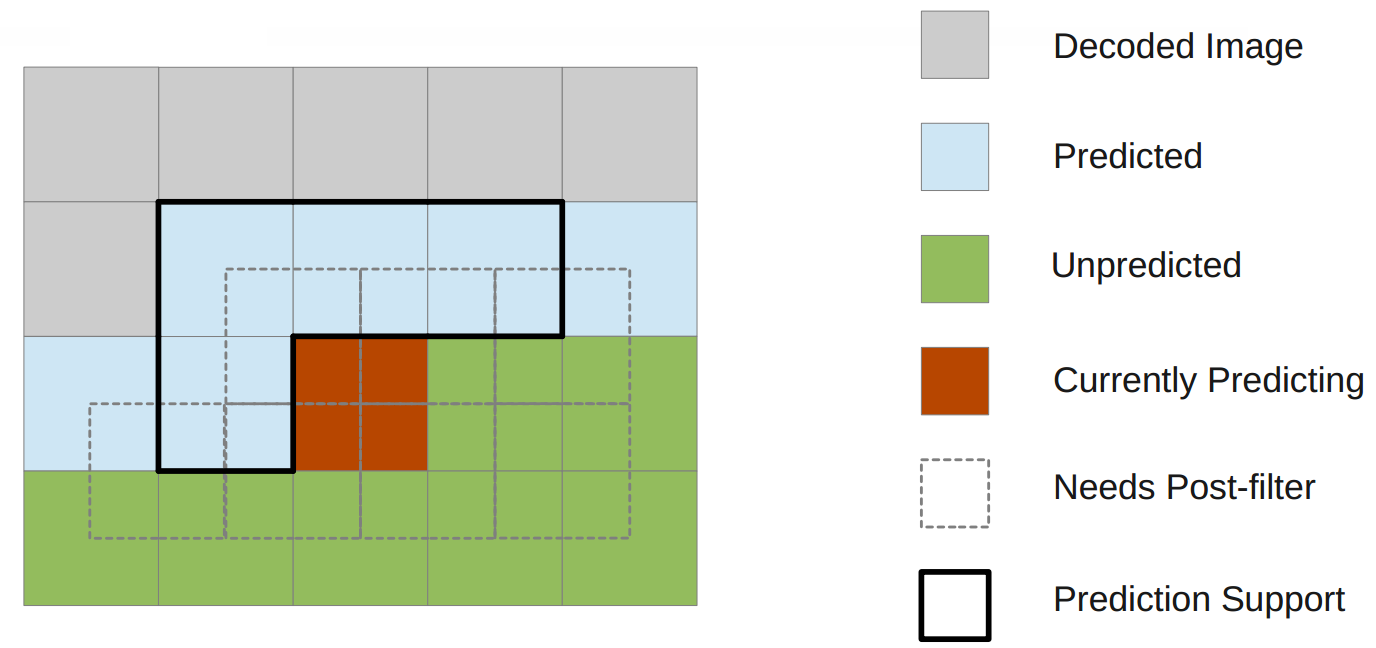
\includegraphics[natwidth=1376,natheight=646,width=4in]{daala_decode.png}
\end{tabular}
\end{center}
\caption[example]{\label{fig:decode} State of blocks in the decode pipeline of
 a codec using lapped transforms. Immediate neighbors of the current block
 (bold lines) cannot be used for spatial prediction as they still require post-
 filtering (dotted lines).}
\end{figure}

\section{RELATED WORK}

Techniques have been proposed for 
The work of Xu, Wu and Zhang considers frequency domain intra prediction using
 non-overlapped blocks\cite{xuwu2009}.
The experimental Daala video codec uses 

describe a framework for generalizing using the frequency domain coefficients was extended by the Daala codec to allow for 

 unlapping post filter appiledthe neighboring \cite{oliv2011}\cite{xuwu2009}

\begin{figure}
\begin{center}
\begin{tabular}{c}
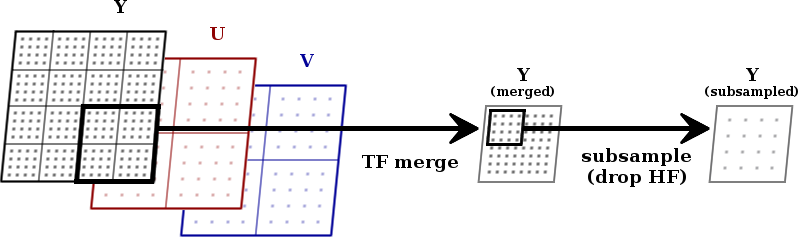
\includegraphics[natwidth=799,natheight=237,width=4in]{CfL-TF.png}
\end{tabular}
\end{center}
\caption[example]{\label{fig:tf} State of blocks in Daala decode pipeline.
 Immediate neighbors of the current block (bold lines) cannot be used for
 spatial prediction as they still require post-filtering (dotted lines).}
\end{figure}

\begin{figure}
\begin{center}
\begin{tabular}{c c c}
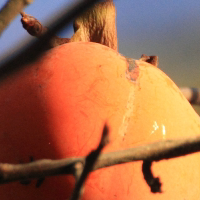
\includegraphics[natwidth=200,natheight=200,width=1.75in]{fruits-orig.png}
&
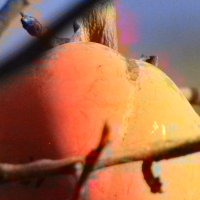
\includegraphics[natwidth=200,natheight=200,width=1.75in]{fruits-intra.png}
&
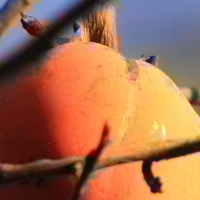
\includegraphics[natwidth=200,natheight=200,width=1.75in]{fruits-cfl.png}
\\
(a) & (b) & (c)
\end{tabular}
\end{center}
\caption[example]{\label{fig:comp} Comparison of (a) the original uncompressed
 image with composite images of (b) reconstructed luma and predicted chroma
 using Daala intra modes and (c) reconstructed luma and predicted chroma using
 Chroma-from-Luma.}
\end{figure}

\section{CHROMA PREDICTION}
\label{sec:chroma}

One technique that looks promising 

\begin{align*}
\alpha & = \frac{I\cdot\displaystyle\sum_i^I x_i\cdot y_i - \displaystyle\sum_i^I x_i\displaystyle\sum_i^I y_i}{I\cdot\displaystyle\sum_i^I x_i\cdot x_i - \left(\displaystyle\sum_i^I y_i\right)^2}, & \beta & = \frac{\displaystyle\sum_i^I y_i -\alpha\cdot\displaystyle\sum_i^I x_i}{I}
\end{align*}

\section{PROPOSED ALGORITHM}
\label{sec:alg}

\section{COMPLEXITY COMPARISON}

\begin{table}
\begin{center}
\begin{tabular}{|c|c|c|c|c|}
\hline
\multirow{2}{*}{Block Size} & \multicolumn{2}{|c|}{Spatial Domain} & \multicolumn{2}{|c|}{Freq. Domain} \\
\cline{2-5}
 & Mults & Adds & Mults & Adds \\
\hline
$N\times N$ & $4*N+2$ & $8*N+3$ & $2*12+2$ & $4*12+3$ \\
\hline
$4\times 4$ & 18 & 35 & 26 & 51 \\
\hline
$8\times 8$ & 34 & 67 & 26 & 51 \\
\hline
$16\times 16$\footnotemark[1] & 66 & 131 & 26 & 51 \\
\hline
\end{tabular}
\end{center}
\caption[example]{\label{fig:comp} Comparison of (a) the original uncompressed
 image with composite images of (b) reconstructed luma and predicted chroma}
\end{table}
\footnotetext[1]{Daala does not currently handle $32\times 32$ luma blocks but will likely add support in the future.}
\cite{valin2013high}

\section{IMPLEMENTATION}

This work is part of the Daala project\cite{DaalaWebsite}.
The full source code, including all of the CfL work described in this paper is
 available in the project git repository\cite{DaalaGit}.

%%%%%%%%%%%%%%%%%%%%%%%%%%%%%%%%%%%%%%%%%%%%%%%%%%%%%%%%%%%%%
%\acknowledgments     %>>>> equivalent to \section*{ACKNOWLEDGMENTS}       
%This unnumbered section is used to identify those who have aided the authors in understanding or accomplishing the work presented and to acknowledge sources of funding.  

%%%%%%%%%%%%%%%%%%%%%%%%%%%%%%%%%%%%%%%%%%%%%%%%%%%%%%%%%%%%%
%%%%% References %%%%%

\bibliography{spie_cfl}   %>>>> bibliography data in report.bib
\bibliographystyle{spiebib}   %>>>> makes bibtex use spiebib.bst

\end{document} 
